\chapter{Methods and Results}
\section{Problem restatement}
We consider every examples in a image QA dataset as a triplet of an image vector, a question of a sequence of word indices, and an answer of a sequence of word indices. We start off by assuming that the answers are all one-word answers, i.e. the length of the answer sequence is always one. The assumption is established based on more than 98\% of the data entries in DAQUAR have only one-word answers. Our goal is to learn a function that takes the input of an image vector and a sequence of word indices, and emits the output of the answer word. 

\section{Our models}
\subsection{GUESS model}
One very simple baseline is to predict the mode based on question type. For example, if the question contains ``how many'' then output ``two.'' This baseline actually works unexpectedly well in DAQUAR dataset.

\subsection{BOW model}
Another baseline is to use the last hidden layer of the Oxford convolutional neural net (4096 dimension) \cite{simonyan14} as an image feature extractor, and use wording embeddings from word2vec. To obtain the sentence-level embedding, we simply sum all the word vectors, i.e. bag-of-words (BOW). We concatenate the image vectors and the word vectors, and send the combined feature into a softmax layer.

\subsection{LSTM sentence model}
Due to the sequential nature of natural languages, researchers have been looking for ways to model sentences using recurrent neural networks. There has been increasing interests in using LSTM to model the embedding vector for a whole sentence. Recently, \cite{sutskever14} uses LSTM as both encoders and decoders in machine translation, and achieved BLEU score \cite{bleu} better than the traditional phrase-based models \cite{luong14}. In our work we use LSTM as our sentence embedding model. At every timestep we input a word vector to the LSTM, and we use the output values of the LSTM at the last timestep as our embedding space representation of the question asked.

\subsection{Image-word model}
We started off the experiment by directly building on top of the LSTM sentence model. In this experiment, we designed a model called the ``image-word model'' because it treats the image as one word of the question. We borrowed the idea of treating the image as the first word of the question from caption generation by \cite{vinyals14}. The difference with caption generation is that here we only output the answer at the last time step.

\begin{enumerate}
	\item We used the last hidden layer of the Oxford convolutional neural net (4096 dimension) \cite{simonyan14} as our visual embedding model.
	\item We use the word2vec embedding model (skip gram) trained from Google News \cite{mikolov13} as our frozen semantic embedding (300 dimension). 
	\item We then treated the image as if it is the first word of the sentence. In order to map the image embedding to our semantic embedding space, we used a linear transformation layer of dimension 4096$\times$300 (similar to \cite{frome13}).
	\item The last time step of the LSTM output is passed to a softmax layer. The final output is a 68-dimension vector representing the probability of the answer being each possible answer classes.
\end{enumerate}

We used the 37 class DAQUAR dataset, so the question and answers will only focus on 37 object classes. We also filtered dataset down to only one-word answers. This simplification trims the possible set of answers to 63 words (including unknown class ``UNK'').
To evaluate the model, we used the plain answer accuracy as well as the Wu-Palmer similarity (WUPS) measure \cite{wu94, malinowski14b}. The WUPS calculates the similarity between two words based on their longest common subsequence in the taxonomy tree. The similarity function takes in a threshold parameter. If the similarity between two words is less than the threshold then zero score will be given to the candidate answer. It reduces to plain accuracy when the threshold equals to 1.0. Following \cite{malinowski14b}, we measure all the models in terms of plain accuracy, WUPS at 0.9 threshold, and WUPS at 0.0 threshold.

To evaluate the results, we also designed a baseline model to avoid over-interpretation. In this model, the images are replaced by randomly generated vectors instead of meaningful graphics. We call this baseline the ``blind model.''

\begin{figure}
\centering
\scalebox{0.9}{
\input{imgword.tex}}
\caption{Image-word model and blind model}
\label{fig:imgword}
\end{figure}

\subsection{Bidirectional image-word model}
The image-word model, which takes in words sequentially in a linear fashion, may not be powerful enough to handle complex sentence structures in the question. At the last timestep it needs to output the answer immediately after reading the last word of the question. In some cases where the hint is revealed at the last timestep, the single direction model may fail to change direction because the previous words have made the model very confident of an answer already. The bidirectional image-word model aims to fix this weakness. It contains two LSTMs. The first one takes the image as the first word and then processes the words sequentially just like the previous model. Moreover, the second LSTM processes the words in a reverse order, together with the hidden state of the first LSTM at that timestep. At the last timestep, the second LSTM takes in the image again. So intuitively, the first timestep gives an ``impression'' of the image, and after knowing the sentence, it checks the image again to confirm the answer. The second LSTM ``sees'' the whole sentence at every timestep, so this model is thought to be better because it considers the entire question for a longer period of time.

\begin{figure}[h]
\centering
\scalebox{0.9}{
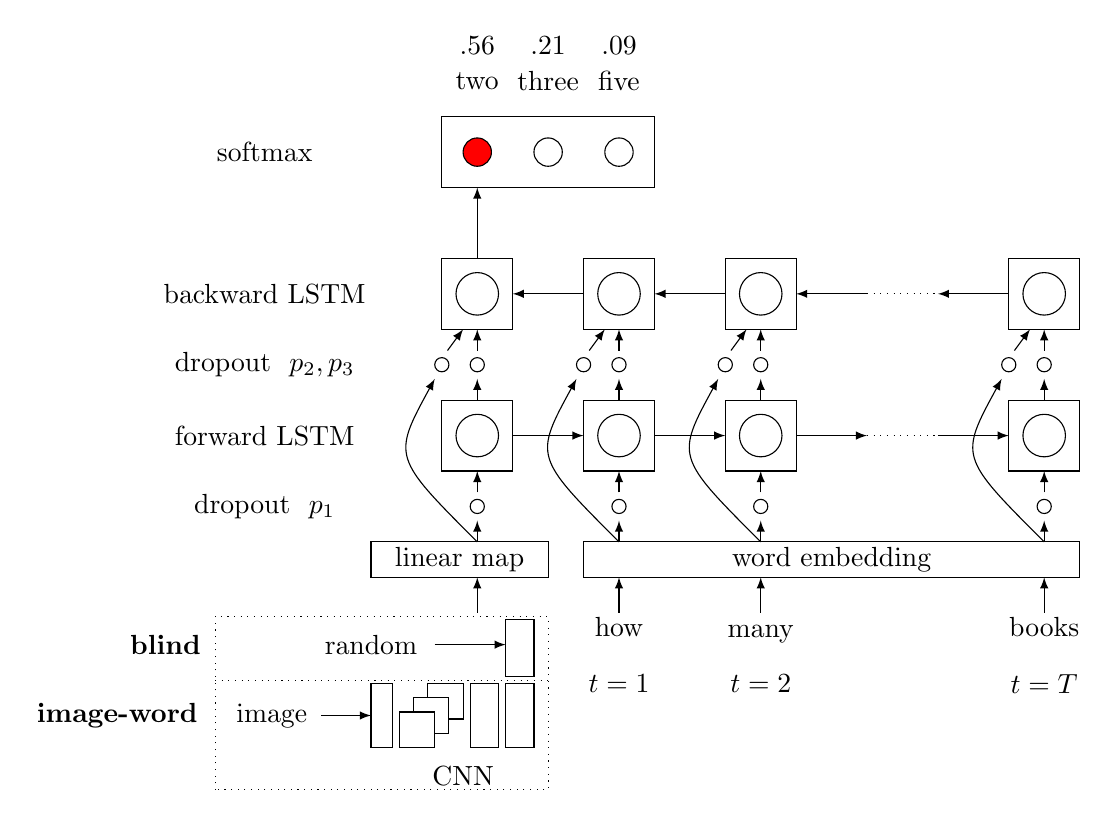
\begin{tikzpicture}[scale=0.9]

\foreach \x in  {5, 7, 9, 13}
{
    \draw (\x,3.0) rectangle (\x+1,4.0);
    \draw (\x+0.5,3.5) circle (0.3cm);
    \draw [-latex](\x+0.5,2.0) -- (\x+0.5,2.3);
    \draw (\x+0.5,2.5) circle (0.1cm);
    \draw (\x-0.0,2.5) circle (0.1cm);
    \draw [-latex](\x+0.5,2.7) -- (\x+0.5,3.0);
}

\foreach \x in  {7, 9, 11, 13}
{
    \draw [latex-](\x-1,3.5) -- (\x,3.5);
}
\draw [dotted] (11,3.5) -- (12,3.5);


\foreach \x in {5.5, 7.5, 9.5, 13.5}
{
    \draw [-latex](\x, 0.0) .. controls (\x-1.2,1.2) .. (\x-0.6,2.3);
    \draw [-latex](\x-0.42, 2.7) -- (\x-0.2, 3.0);
}

\foreach \x in  {5, 7, 9, 13}
{
    \draw (\x,1) rectangle (\x+1,2);
    \draw (\x+0.5,1.5) circle (0.3cm);
    \draw [-latex](\x+0.5,0) -- (\x+0.5,0.3);
    \draw (\x+0.5,0.5) circle (0.1cm);
    \draw [-latex](\x+0.5,0.7) -- (\x+0.5,1);
}

\foreach \x in  {7, 9, 13}
{
    \draw [-latex](\x+0.5,-1) -- (\x+0.5,-0.5);
}

\foreach \x in  {7, 9, 11, 13}
{
    \draw [-latex](\x-1,1.5) -- (\x,1.5);
}

\path (7.5,-2) node[draw=none] (t0) {$t=1$};
\path (9.5,-2) node[draw=none] (t1) {$t=2$};
\path (13.5,-2) node[draw=none] (tT1) {$t=T$};
\draw [dotted] (11,1.5) -- (12,1.5);

\path (7.5,-1.2) node[draw=none] (w1) {how};
\path (9.5,-1.3) node[draw=none] (w2) {many};
\path (13.5,-1.2) node[draw=none] (w3) {books};
\path (2.5,0.5) node[draw=none] (drop) {dropout $~p_1$};
\path (2.5,1.5) node[draw=none] (lstm1) {forward LSTM};
\path (2.5,2.5) node[draw=none] (drop) {dropout $~p_2, p_3$};
\path (2.5,3.5) node[draw=none] (lstm1) {backward LSTM};
\draw (7, -0.5) rectangle (14, 0);

\draw (5,5) rectangle (8,6);
\draw[fill=red] (5.5,5.5) circle (0.2cm);
\draw (6.5,5.5) circle (0.2cm);
\draw (7.5,5.5) circle (0.2cm);
\path (2.5,5.5) node[draw=none] (logit) {softmax};
\path (5.5,6.5) node[draw=none] (logit2) {two};
\path (6.5,6.5) node[draw=none] (logit3) {three};
\path (7.5,6.5) node[draw=none] (logit5) {five};
\path (5.5,7) node[draw=none] (logit2) {.56};
\path (6.5,7) node[draw=none] (logit3) {.21};
\path (7.5,7) node[draw=none] (logit5) {.09};
\draw [-latex] (5.5,4) -- (5.5,5);

\draw (4,-0.5) rectangle (6.5, 0);
\path (5.25,-0.25) node[draw=none] (imgMap) {linear map};

\draw (4.0, -2.9) rectangle (4.3, -2);
\draw[fill=white] (4.8, -2.5) rectangle (5.3, -2);
\draw[fill=white] (4.6, -2.7) rectangle (5.1, -2.2);
\draw[fill=white] (4.4, -2.9) rectangle (4.9, -2.4);
\draw (5.4, -2.9) rectangle (5.8, -2);
\draw (5.9, -2.9) rectangle (6.3, -2);
\draw (5.9, -1.9) rectangle (6.3, -1.1);
\draw [-latex] (5.5, -1.0) -- (5.5, -0.5);

\draw [-latex] (4.9,-1.45) -- (5.9, -1.45);
\draw [-latex] (3.3,-2.45) -- (4.0, -2.45);
\path (4.0,-1.45) node[draw=none] (random) {random};
\path (2.6,-2.45) node[draw=none] (image) {image};
\path (1.1,-1.45) node[draw=none] (blind) {\textbf{blind}};
\path (0.42,-2.45) node[draw=none] (image-word) {\textbf{image-word}};
\path (5.3,-3.3) node[draw=none] (cnn) {CNN};
\draw [dotted] (1.8,-1.95) -- (6.5, -1.95);
\draw [dotted] (1.8,-3.5) rectangle (6.5, -1.05);

\path (10.5,-0.25) node[draw=none] (Wemb) {word embedding};


\end{tikzpicture}}
\caption{Bidirectional image-word model and blind model}
\label{fig:imgword}
\end{figure}

\subsection{Image-word ranking model}
The softmax layer can be replaced by other types of loss. The ranking loss is very popular in recent question answering literature because it is very fast to train. This type of model outputs a vector that is the nearest neighbour of the answer word in the semantic embedding. The error function uses the pair-wise ranking loss \cite{weston10}, defined below:

\begin{equation}
\sum\limits_{\+y} \sum\limits_{i \neq j} \max \{0, \alpha-s(\+y, \+a_j) + s(\+y, \+a_i) \}
\end{equation}

$\+y$ and $\+a$ are both vectors in the answer embedding space. $\+y$ is the output of the model, and $\+a_j$ is the correct answer for the question, and $\+a_i$ is one of any possible answers. $s(\cdot, \cdot)$ denotes the similarity measure of two vectors. It is usually implemented as the cosine similarity in high dimensional spaces: 
\begin{equation}
s(\+x, \+y) = \dfrac{\+x \cdot \+y} {\norm{\+x} \norm{\+y}}
\end{equation}

This error function will penalize the model if the right answer is not winning over other wrong answers by a certain margin $\alpha$. It is a widely used in ranking image descriptions \cite{kiros14b}. The ranking loss effectively replaces the softmax layer, and the hidden dimension of the LSTM need to match with the word embedding dimension. 

\subsection{DAQUAR results}
\label{sec:daquar_results}
Table~\ref{tab:daquar_results} summarizes the performance of our proposed models and our baselines. First, our models win by a large margin compared to the results from the publisher of the DAQUAR dataset. Second, we argue that most gain in accuracy results from a good sentence embedding, because the blind model has almost the same accuracy compared to the image-word model. Third, the bidirectional model further improves the performance by a small amount. Lastly, the ranking loss model does not outperform the softmax model. Although the training is much faster even with a smaller learning rate, it achieves lower accuracy because it tends to overfit the training set too quickly.

In Figure~\ref{fig:imgword+blind}, we further discovered the some weak visual ability by a direct comparison of test examples. We observed that the image-word model seems to perform better on questions centered on dominant objects or dominant colours, but does not seem to learn how to count.

\begin{figure}
    \centering
    \footnotesize
    \begin{subfigure}[t]{0.3\textwidth}
            \includegraphics[width=\textwidth]{bed_vs_table.jpg}
            Q193: what is the largest object ?\\
            Image-word: table (0.576)\\
            Blind: bed (0.440)\\
            Ground truth: table
            \caption{The question gives no extra clue of the class of the object. The visual model recognizes the correct object through the shape.}
    \end{subfigure}%
    \quad
    \begin{subfigure}[t]{0.3\textwidth}
            \includegraphics[width=\textwidth]{fridge_vs_toilet.jpg}
            Q212: what is the object left of the room divider ?\\
            Image-word: toilet (0.3973), sink (0.1367), towel (0.1323)\\
            Blind: refridgerator (0.5318)\\
            Ground truth: door
            \caption{The visual model recognizes the correct scene.}
    \end{subfigure}
    \quad
    \begin{subfigure}[t]{0.3\textwidth}
            \includegraphics[width=\textwidth]{three_vs_three.jpg}
            Q1615: how many pictures are there on the wall ?\\
            Image-word: three (0.4518)\\
            Blind: three (0.6047)\\
            Ground truth: seven
            \caption{No evidence shows that image-word model learns how to count.}
    \end{subfigure}
    \caption{Direct comparison between the image-word model and the blind model.}
    \label{fig:imgword+blind}
\end{figure}

\begin{table}[h]
\centering
\caption{DAQUAR results}
\label{tab:daquar_results}
\begin{minipage}{10.5cm}
%{6cm}
\begin{tabular}{l l l l l l l l}
\toprule
                 & \textbf{Accuracy} & \textbf{WUPS 0.9} & \textbf{WUPS 0.0}\\
\midrule
\textbf{2-IMGWD}\footnote{Bidirectional image-word model} & \textbf{0.3276} & \textbf{0.3298} & 0.7272\\
\textbf{IMGWD}\footnote{Image-word model}   & 0.3188   & 0.3211 & \textbf{0.7279}\\
\textbf{IMGWD-RK}\footnote{Image-word ranking model}   & 0.2787 & 0.2782 & 0.7074\\
\midrule
\textbf{BLIND}\footnote{Single-direction blind model}   & 0.3051   & 0.3069 & 0.7229\\
\textbf{RANDWD}\footnote{Single-direction model with random word embedding}  & 0.3036   & 0.3056 & 0.7206\\
\textbf{BOW}\footnote{Bag-of-words model}     &  0.2299  & 0.2340 & 0.6907\\
\textbf{GUESS}\footnote{Guess ``two'', ``white'', and ``table'', depending on question type}   & 0.1785   & 0.1823       & 0.6874\\
\textbf{MultiWorld \cite{malinowski14b}} & 0.1273 & 0.1810 & 0.5147\\
\midrule
\textbf{HUMAN} & 0.6027 & 0.6104 & 0.7896\\
\bottomrule
\end{tabular}
\end{minipage}
\end{table}

\section{COCO-QA dataset}
From DAQUAR results, we see that although our models have improved the answer accuracy by a lot compared to the previous attempt, the blind version of the model can do almost equally well, suggesting that the image features from the CNN are not very useful. Since 1500 images are a very small dataset, maybe it is worthwhile for us to build a larger dataset so that the neural networks can be trained more robustly.

Manually annotating pictures with QA pairs requires large amount of time, capital, and tools. We propose to use currently massively available image description dataset and convert descriptions into QA forms. This method is cheap, fast, and scalable; however the drawback is that the quality of automatically generated questions is unforeseeable. There lacks a measure to test how sensical the questions are overall.

We used recently released Microsoft Common Objects in COntext (MS-COCO) \cite{mscoco} dataset, which contains 100K images and 500K sentence descriptions, and converted the descriptions into QA pairs. We only considered three types of questions: object, number, and colour, and only single-word answers.

\subsection{Question conversion algorithms}
Here we present an algorithm that converts sentences into different types of questions.

\subsubsection{Object-type questions}
First, we consider asking an object using ``what'' or ``who''. This involves replacing the actual object with a ``what'' in the sentence, and then transforming the sentence structure so that the ``what'' appears in the front of the sentence. The algorithm below assumes that the input is a sentence in the form of a syntactic tree, and the output is a question in the form of a syntactic tree.

The entire algorithm has the following stages:
\begin{enumerate}
\item Split long sentences into simple sentences (see Algorithm~\ref{alg:splitcc}). \\
For question generation task, sentences need not to be very descriptive, and shorter the original sentences are, more readable the questions will be. Moreover, the wh-words that are found in sub-sentences or clauses will less likely be able to perform wh-movement \cite{borsley99}. Here we only consider a simple case that is when two sentences are joined together with a conjunctive word ``and''. We split the orginial sentences into two independent sentences.
 For example, ``There is a cat and the cat is running.'' will be split as ``There is a cat.'' and ``The cat is running.''
\item Change indefinite determiners to definite determiners (see Algorithm~\ref{alg:indef2def}).\\
Asking questions on a specific instance of the subject requires changing the determiner into definite form ``the''. For example, ``\textbf{A} boy is playing \underline{baseball}.'' will have ``the'' instead of ``a'' in its question form: ``\underline{What} is \textbf{the} boy playing?''.

\item Traverse the sentence and identify potential answers (see Algorithm \ref{alg:traverseWhat}). \\
We traverse the tree structure and identify answers that belong to certain word categories. Then we replace the answer with a question word ``what'' or ``who'' depending on the object type.

\item Perform wh-movement with some constraints (see Algorithm~\ref{alg:whmove}). \\
For English language, questions tend to start with interrogative words such as ``what'' and ``who''. The algorithm needs to move the verb as well as the ``wh-'' constituent to the front of the sentence. However, not all sentences allow such transformation. In this work we consider the following constraints:
\begin{enumerate}
\item A-over-A principle\\
The A-over-A principle was first discovered by Chomsky \cite{chomsky73}. For example, ``I am talking to John and \textbf{Bill}'' cannot be transformed into ``*Who am I talking to John and'' because ``Bill'' is an noun phrase (NP) constituent that is under another NP ``John and Bill''. Therefore, the child NP cannot be removed from the parent NP in the wh-movement.
\item Clauses\\
Except for a few cases, interrogative words in clauses usually cannot be moved to the front of the sentences. For example, ``I am riding a motorcycle that \textbf{Bill} wanted.'' cannot be transformed into ``*Who am I riding a motorcycle that wanted.''. In the future, there is a need to separate the original sentences into two: ``I am riding a motorcycle.'' and ``Bill wanted the motorcycle.''. For now, wh-word in the clauses will terminate the wh-movement process and our algorithm will only output sentences like ``I am riding a motorcycle that \textbf{who} wanted?''.
\end{enumerate}
\end{enumerate}

The entry point of the overall algorithm is shown in Algorithm~\ref{alg:askWhat}. Figure~\ref{fig:whmove} illustrates these procedures with tree diagrams. We used WordNet \cite{wordnet} and NLTK software package \cite{nltk} to lemmatize verbs and to get noun categories. We used Stanford parser \cite{klein03} to obtain syntatic structure of the original sentence.
\begin{algorithm}
\caption{Split compound sentences}
\label{alg:splitcc}
\begin{algorithmic}[1]
\Require Root of the syntactic tree of the original sentence
\Ensure List of roots of syntactic trees of split sentences
\Procedure{SplitCC}{root}
\State node $\gets$ root.children$[0]$ \Comment{Search directly from ``S'' node}
\If{node is ``S'' and it has more than 3 children}
    \If{All children are ``S'' or ``CC'' and ``CC''s are always in between two ``S''s}
        \State \Return each ``S'' child
    \EndIf
\EndIf
\EndProcedure
\end{algorithmic}
\end{algorithm}

\begin{algorithm}
\caption{Replace indefinite determiners to definite determiners}
\label{alg:indef2def}
\begin{algorithmic}[1]
\Require Root of the syntactic tree with wh-word in the original place
\Ensure Root of the syntactive tree with wh-word in the front
\Procedure{SwitchDefDet}{root}
\State node $\gets$ \Call{DFS}{root, ``NP''} \Comment{Depth-first search for the subject in the sentence}
\State node $\gets$ \Call{DFS}{node, ``DT''} \Comment{Depth-first search for the determiner of the subject}
\If{node.text = ``a'' \textbf{or} node.text = ``an''}
    \State node.text $\gets$ ``the''
\EndIf
\State \Return root
\EndProcedure
\end{algorithmic}
\end{algorithm}

\begin{algorithm}
\caption{Identify object-type answers}
\label{alg:traverseWhat}
\begin{algorithmic}[1]
\Require Root of the syntactic tree of the original sentence
\Ensure List of roots of the syntactic trees with answers replaced by ``what''
\Procedure{TraverseWhat}{root, results}
\For{child $\in$ node.children}
    \State \Call{TraverseWhat}{child, results}
\EndFor
\If{node is``NP'' and node's children contains a noun is of category\\
    \hspace{\algorithmicindent} \hspace{\algorithmicindent} animal, artifact, body, food, object, plant, possession, shape, person}
    \State answer $\gets$ noun
    \State whatNode $\gets$ Node(class=``WP'', text=``who/what'', children=$[\ ]$)
    \State Replace answer with Node(class=``WHNP'', text=``'',  children=$[$whatNode$]$)
    \State Insert the modified root into roots list
\EndIf
\EndProcedure
\end{algorithmic}
\end{algorithm}

\begin{algorithm}
\caption{Wh-movement}
\label{alg:whmove}
\begin{algorithmic}[1]
\Require Root of the syntactic tree with wh-word in the original place
\Ensure Root of the syntactive tree with wh-word in the front
\Procedure{Wh-movement}{root}

\State Check if the sentence contains a verb-phrase. If no, terminate.
\State Check if ``WHNP'' is under ``SBAR'' or ``NP''. If yes, terminate.

\State verbFront $\gets$ \textbf{null}
\If{the verb is any tensed form of ``be'' or ``have done'', or is a modifier e.g. ``will''}
    \State verbFront $\gets$ verb
    \State Remove verb from its parent
\Else
    \State verbFront $\gets$ Node(class=verb.class, text=``does/do/did'', children=$[]$)
    \State verb $\gets$ \Call{Lemmatize}{verb}
\EndIf

\State Remove WHNP from its parent
\State S\_old $\gets$ root.children$[0]$
\State S\_old.children.insert(verbFront, 0) \Comment{Insert verbFront as the first child of S\_old}
\State S\_new $\gets$ Node(class=``S'', text=``'', children=$[$WHNP, S\_old$]$)
\State root.children $\gets [$S\_new$]$
\State \Return root
\EndProcedure
\end{algorithmic}
\end{algorithm}

\begin{algorithm}
\caption{Generate object-type questions}
\label{alg:askWhat}
\begin{algorithmic}[1]
\Require Root of the syntactic tree of the original sentence
\Ensure List of roots of the syntactic trees of generated questions

\Procedure{AskWhat}{Root}
\State \Call{SwitchDefDet}{root}
\For {r $\in$ \Call{SplitCC}{root}}
    \State roots $\gets [\ ]$, \Call{TraverseWhat}{r, roots}
    \For {r2 $\in$ roots}
        \State \textbf{yield return} \Call{Wh-movement}{r2}
    \EndFor
\EndFor
\EndProcedure
\end{algorithmic}
\end{algorithm}


\begin{figure}[h]
    \centering
    \small
    \begin{subfigure}[t]{0.45\textwidth}
        \caption{Step 1: Parse the sytactic structure.}
        \centering
        \scalebox{0.8}{
        \Tree [.S [.NP [.DET a ] [.N man ] ] [.VP [.V is ] [.NP [.VBG riding ] [.NP [.DET a ] [.N horse ] ] ] ] ]}
        \vspace{5mm}
    \end{subfigure}
    \quad
    \begin{subfigure}[t]{0.45\textwidth}
        \caption{Step 2: Change determiner.}
        \centering
        \scalebox{0.8}{
        \Tree [.S [.NP [.DET \textbf{the} ] [.N man ] ] [.VP [.V is ] [.NP [.VBG riding ] [.NP [.DET a ] [.N horse ] ] ] ] ]}
        
        \vspace{5mm}
    \end{subfigure}
    \begin{subfigure}[t]{0.45\textwidth}
        \caption{Step 3: Find the answer of the question.}
        \centering
        \scalebox{0.8}{
        \Tree [.S [.NP [.DET the ] [.N man ] ] [.VP [.V is ] [.NP [.VBG riding ] [.NP [.DET \textbf{a} ] [.N \textbf{horse} ] ] ] ] ]}
        \vspace{5mm}
    \end{subfigure}
    \quad
    \begin{subfigure}[t]{0.45\textwidth}
        \caption{Step 4: Replace the answer with ``what''.}
        \centering
        \scalebox{0.8}{
        \Tree [.S [.NP [.DET the ] [.N man ] ] [.VP [.V is ] [.NP [.VBG riding ] [.NP [.DET \sout{a} ] [.N \sout{horse} ] ] ] ] ]}
        \vspace{5mm}
    \end{subfigure}
    \begin{subfigure}[t]{0.45\textwidth}
        \caption{Step 4: Replace the answer with ``what''.}
        \centering
        \scalebox{0.8}{
        \Tree [.S [.NP [.DET the ] [.N man ] ] [.VP [.V is ] [.NP [.VBG riding ] [.WHNP [.WP \textbf{what} ] ] ] ] ]}
        \vspace{5mm}
    \end{subfigure}
    \quad
    \begin{subfigure}[t]{0.45\textwidth}
        \caption{Step 5: Perform WH-fronting.}
        \centering
        \scalebox{0.8}{
        \Tree [.S [.WHNP [.WP what ] ] [.S [.V is ] [.NP [.DET the ] [.N man ] ] [.VP [.V \sout{is} ] [.NP [.VBG riding ] [.WHNP [.WP \sout{what} ] ] ] ] ] ]}
        \vspace{5mm}
    \end{subfigure}
    \caption{
        Example: ``A man is riding a \textbf{horse}'' $=>$ ``\textbf{What} is \textbf{the} man riding?''}
    \label{fig:whmove}
\end{figure}

\subsubsection{Number-type questions}
To generate ``how many'' types of questions, we follow a similar procedure as the previous algorithms, except a different way to identify potential answers. This time, we need to extract numbers from original sentences. Splitting compound sentences, changing determiners, and wh-movement parts remain the same. Algorithm~\ref{alg:traverseHowMany}, \ref{alg:askHowMany} shows an detailed algorithm.

\begin{algorithm}[h]
\caption{Identify number-type answers}
\label{alg:traverseHowMany}
\begin{algorithmic}[1]
\Require Root of the syntactic tree of the original sentence
\Ensure List of roots of the syntactic trees with answers replaced by ``how many''
\Procedure{TraverseHowMany}{root, results}
\For{child $\in$ node.children}
    \State \Call{TraverseHowMany}{child, results}
\EndFor
\State answer $\gets$ \textbf{null}
\If{node is ``NP'' and node's children contains number}
    \State howNode $\gets$ Node(class=``WRB'', text=``how'', children=$[\ ]$)
    \State manyNode $\gets$ Node(class=``JJ'', text=``many'', children=$[\ ]$)
    \State parent $\gets$ Node(class=``WHNP'', text=``'', children=$[$howNode, manyNode$]$)
    \State Replace the number node with parent
    \State Insert the modified root into results list
\EndIf
\EndProcedure
\end{algorithmic}
\end{algorithm}

\begin{algorithm}[h]
\caption{Generate number-type questions}
\label{alg:askHowMany}
\begin{algorithmic}[1]
\Require Root of the syntactic tree of the original sentence
\Ensure List of roots of the syntactic trees of generated questions

\Procedure{AskHowMany}{Root}
\State results $\gets [\ ]$
\State \Call{SwitchDefDet}{root}
\For {r $\in$ \Call{SplitCC}{root}}
    \State roots $\gets [\ ]$, \Call{TraverseHowMany}{r, roots}
    \For {r2 $\in$ roots}
        \State \textbf{yield return} \Call{Wh-movement}{r2}
    \EndFor
\EndFor
\EndProcedure
\end{algorithmic}
\end{algorithm}

\subsubsection{Colour-type questions}
Compared to the previous two question types, colour-type questions are much easier to generate. It only requires locating the colour adjective and the noun which the adjective attaches to. Then it simply forms a sentence ``What is the colour of the object'' with the ``object'' replaced by the actual noun. The tree traversal is also similar to previously presented algorithms so the implementation details are omitted.

\subsection{Reducing rare answers}
Here we impose a hard constraint such that all answers must at least appear $L$ times in the dataset. In the 6.6K dataset, $L=5$, and in the full dataset, $L=20$. The reason of imposing this constraint is that otherwise we would end up with many answers that only appear once in the training set. This will significantly increase the difficulty of the task.

\subsection{Reducing common answers}
Besides creating more data, the other main motivation here is to reduce the performance of a model that simply guesses for the three most common answers (i.e. mode guessing) for each type of question (e.g. ``man'', ``two'', ``white''). Therefore, additional constraint needs to be imposed to reduce the common answers. The probability of enrolling an question-answer pair $(q, a)$ is:
\begin{equation}
p(q, a) = \left\{ \begin{array}{cl}
1 &\mbox{ if \text{count}$(a)$ $\le U$ } \\
\exp\left(-\dfrac{\text{count}(a) - U}{2U}\right) &\mbox{ otherwise }
\end{array} \right.
\end{equation}
where $U=100$ in both the 6.6K dataset and the full dataset. This will penalize answers for appearing more than $U$ times while still preserve the rank of the most common answers.

\subsection{Question statistics}
With the automatic question generation technique described above, we gathered a dataset from the MS-COCO dataset. We name this dataset to be COCO-QA dataset. Table~\ref{tab:cocoqa_stats} presents some important statistics of COCO-QA, with comparison to DAQUAR. The full dataset is considered to be harder than DAQUAR, because it has more possible answer classes and lower guess baseline accuracy. However, COCO-QA contains 60 times more images and 20 times more question-answer pairs, so it is more suitable to deep learning approaches.

\begin{table}[h]
\centering
\caption{General statistics of COCO-QA and DAQUAR}
\label{tab:cocoqa_stats}
\begin{minipage}{14cm}
\begin{tabular}{c c c c c}
\toprule
\textbf{Dataset} & \textbf{\# Images} & \textbf{\# Questions} & \textbf{\# Answers\footnote{Number of answers present in the training set plus the unknown ``UNK'' class}} & \textbf{GUESS accuracy}\footnote{Guess the three most common answers depending on question types}\\
\midrule
DAQUAR-37\footnote{Trimmed to include only single-word answer}  &  795+654\footnote{``+'' denotes train-test split}  & 3825+3284  & 63     & 0.1885\\
DAQUAR-894\footnote{Trimmed to include only single-word answer}  &  795+654  & 6149+5076  & 412    & 0.1180\\
COCO-QA 6.6K & 3.6K+3K      & 14K+11.6K  & 298        & 0.1157         \\
COCO-QA Full & 80K+20K      & 177K+83K & 794           & 0.0347\\
\bottomrule
\end{tabular}
\end{minipage}
\end{table}

\begin{table}[h]
\centering
\caption{
COCO-QA and DAQUAR question type break-down (numbers inside the brackets denote the proportion with regard to the entire dataset)}
\begin{tabular}{c c c c c c}
\toprule
\textbf{Dataset}      &         & \textbf{Object} & \textbf{Number} & \textbf{Colour} & \textbf{Total}  \\
\midrule
\textbf{DAQUAR-37}    & Train   & 2814 (0.7357)   & 903 (0.2361)    & 108 (0.0282)   & 3825 (1.0000)   \\
                      & Test    & 2406 (0.7326)   & 779 (0.2372)    & 99 (0.0301)    & 3284 (1.0000)   \\
\midrule
\textbf{DAQUAR-894}   & Train   & 5131 (0.8344)   & 903 (0.1469)    & 115 (0.0187)   & 6149 (1.0000)   \\
                      & Test    & 4194(0.8262)    & 779(0.1535)     & 103(0.0203)    & 5076(1.0000)    \\
\midrule
\midrule
\textbf{COCO-QA 6.6K} & Train   & 10759 (0.7641)  & 1134 (0.0805)   & 2187 (0.1553)  & 14080 (1.0000)  \\
                      & Test    & 8850 (0.7645)   & 939 (0.0811)    & 1878 (0.1544)  & 11576 (1.0000)  \\
\midrule
\textbf{COCO-QA Full} & Train   & 155888 (0.8824) & 7213 (0.0408)   & 13561 (0.0768) & 176662 (1.0000) \\
                      & Test    & 73483  (0.8875) & 3181 (0.0384)   & 6135 (0.0741)  & 82809 (1.0000)  \\
\bottomrule
\end{tabular}
\end{table}

\subsection{Question quality}
Assessing the exact quality of the generated question is not feasible. We either need human workers to manually go through the entire dataset, or we need to have a program that knows a perfect grammar. There are mainly two sources of errors: first is caused by incorrect sentence structures produced by the Stanford parser and second is caused by our algorithms. By going through the first 100 samples of the generated questions ourself, we found that 81\% of the questions are grammatical, and 63\% of the questions are meaningful. This precision can be further tuned up by employing more strict question generation rules (i.e. lowering the recall). We will discuss a few future work items in Chapter \ref{future}. But the two raw statistics above show that we have a functional question generation algorithm that can be used for our QA learning task.

\subsection{Learning results}
We applied the same models, the single directional and the bi-directional image-word model, on the COCO-QA dataset. Table~\ref{tab:cocoqa_results} summarizes the results. We further computed the accuracy in each question category in Table~\ref{tab:cocoqa_acc_breakdown}.
\begin{table}[h]
\centering
\caption{COCO-QA results}
\label{tab:cocoqa_results}
\begin{tabular}{c c c c | c c c}
\toprule
                 &          &\textbf{6.6K}&             &          &\textbf{Full}&           \\
\midrule
                 & \textbf{Acc.}     & \textbf{WUPS 0.9}   & \textbf{WUPS 0.0}       & \textbf{Acc.}     & \textbf{WUPS 0.9}   & \textbf{WUPS 0.0}     \\
\midrule
%\hline
\textbf{2-IMGWD} & \textbf{0.3358} & \textbf{0.3454} & \textbf{0.7534} & \textbf{0.3208} & \textbf{0.3304} & \textbf{0.7393} \\
\textbf{IMGWD}   & 0.3260   & 0.3357     & 0.7513       & 0.3153   & 0.3245     & 0.7359     \\
\midrule
%\hline
\textbf{BOW}     & 0.1910   & 0.2018     & 0.6968       & 0.2365   & 0.2466     & 0.7058     \\
\textbf{RANDWD}  & 0.1366   & 0.1545     & 0.6829       & 0.1971   & 0.2058     & 0.6862     \\
\textbf{BLIND}   & 0.1321   & 0.1396     & 0.6676       & 0.2517   & 0.2611     & 0.7127     \\
\textbf{GUESS}   & 0.1157   & 0.1608     & 0.6893       & 0.0347   & 0.0609     & 0.6376      \\
\bottomrule
%\hline
\end{tabular}
\end{table}

\begin{table}[h]
\centering
\caption{Full COCO-QA accuracy per category break-down}
\label{tab:cocoqa_acc_breakdown}
\begin{tabular}{c c c c c}
\toprule
                   & \textbf{Object} & \textbf{Number} & \textbf{Colour}  & \textbf{Total}  \\
\midrule
\textbf{2-IMGWD}   & \textbf{0.3139} & \textbf{0.4233} & 0.3600          & \textbf{0.3208} \\
\textbf{IMGWD}     & 0.3078          & 0.4189          & \textbf{0.3604} & 0.3153         \\
\midrule
\textbf{BOW}       & 0.2273          & 0.3398          & 0.3027          & 0.2365          \\
\textbf{BLIND}     & 0.2389          & 0.3713          & 0.3539          & 0.2517          \\
\textbf{RANDWD}    & 0.1828          & 0.3836          & 0.2885          & 0.1971          \\
\textbf{GUESS}     & 0.0138          & 0.3024          & 0.1446          & 0.0347          \\
\bottomrule
\end{tabular}
\end{table}

First, the bi-directional image-word model is still the best model, which is consistent with our DAQUAR results. Second, the model has reasonable visual ability answering object-type questions, as the bi-directional model wins 7\% compared to the blind model. Since the CNN was originally trained for the ImageNet  challenge \cite{ilsvrc14}, and the distribution of object types in COCO is closer to ImageNet, the image feature from the CNN is more useful here than in DAQUAR. Third, the model ``guesses'' the colour of an object almost entirely from a good word embedding and sentence modelling, since there is only 0.6\% gain in colour-type questions by adding image features. Fourth, the model has very limited counting ability since the guess baseline (always guessing ``two'') achieves 30.24\%, whereas the bidirectional model achives 42.33\%. In short conclusion, in our new COCO-QA dataset, we show that our models perform much better than simply guessing the modes. In particular, our model is doing reasonable on object-type questions even with a large number of answers classes present, but it clearly needs further improvement in counting and recognizing colours.

\begin{figure}
\footnotesize
\begin{subfigure}[t]{0.3\textwidth}
    \includegraphics[width=\textwidth, height=.7\textwidth]{formation1.jpg}
    Q683: how many military jet fighter is flying in formation alongside a 1 military propeller pilot ?\\
    2-IMGWD: four (0.402)\\
    Ground truth: one\\
\end{subfigure}
\quad
\begin{subfigure}[t]{0.3\textwidth}
    \includegraphics[width=\textwidth, height=.7\textwidth]{formation2.jpg}
    Q7746: how many airplanes are flying up in the air in formation ?\\
    2-IMGWD: four (0.334)\\
    Ground truth: four\\
\end{subfigure}
\quad
\begin{subfigure}[t]{0.3\textwidth}
    \includegraphics[width=\textwidth, height=.7\textwidth]{formation3.jpg}
    Q8473: how many jets in the sky in a flying formation ?\\
    2-IMGWD: four (0.329)\\
    Ground truth: eight\\
\end{subfigure}

\begin{subfigure}[t]{0.3\textwidth}
    \includegraphics[width=\textwidth, height=.7\textwidth]{giraffe1.jpg}
    Q8325: how many giraffes are partially hidden in brush and sticking their necks out ?\\
    2-IMGWD: three (0.302)\\
    Ground truth: two
\end{subfigure}
\quad
\begin{subfigure}[t]{0.3\textwidth}
    \includegraphics[width=\textwidth, height=.7\textwidth]{giraffe2.jpg}
    how many giraffes in grassy field next to trees ?\\
    2-IMGWD: three (0.361)\\
    Ground truth: three
\end{subfigure}
\quad
\begin{subfigure}[t]{0.3\textwidth}
    \includegraphics[width=\textwidth, height=.7\textwidth]{giraffe3.jpg}
    Q13103: how many giraffes standing together and eating near some trees ?\\
    2-IMGWD: three (0.317)\\
    Ground truth: five
\end{subfigure}

\caption{Counting ability of the image-word model: the outputs are strongly dependent on the types of object asked.}
\label{fig:cocoqa_number}
\end{figure}

\begin{figure}\footnotesize
\begin{subfigure}[t]{0.3\textwidth}
    \includegraphics[width=\textwidth, height=.7\textwidth]{two1.jpg}
    Q44: an open food container box with how many unknown food items ?\\
    2-IMGWD: two (0.258)\\
    Ground truth: four
\end{subfigure}
\quad
\begin{subfigure}[t]{0.3\textwidth}
    \includegraphics[width=\textwidth, height=.7\textwidth]{two2.jpg}
    Q47: the beautiful dessert waiting to be shared by how many people ?\\
    2-IMGWD: two (0.450)\\
    Ground truth: two
\end{subfigure}
\quad
\begin{subfigure}[t]{0.3\textwidth}
    \includegraphics[width=\textwidth, height=.7\textwidth]{two3.jpg}
    Q1016: how many motor cycle racers posing on their parked bikes ?\\
    2-IMGWD: two (0.460)\\
    Ground truth: three
\end{subfigure}

\caption{Counting ability of the image-word model: the model outputs ``two'' when it is not certain about the objects.}
\end{figure}

\begin{figure}\footnotesize
\begin{subfigure}[t]{0.3\textwidth}
    \includegraphics[width=\textwidth, height=.7\textwidth]{banana1.jpg}
    Q10371: what is the colour of the bananas ?\\
    2-IMGWD: green (0.488)\\
    Ground truth: green\\
\end{subfigure}
\quad
\begin{subfigure}[t]{0.3\textwidth}
    \includegraphics[width=\textwidth, height=.7\textwidth]{banana2.jpg}
    Q16954: what is the colour of the bananas ?\\
    2-IMGWD: green (0.488)\\
    Ground truth: yellow\\
\end{subfigure}
\quad
\begin{subfigure}[t]{0.3\textwidth}
    \includegraphics[width=\textwidth, height=.7\textwidth]{banana3.jpg}
    Q5594: what is the color of the bananas ?\\
    2-IMGWD: green (0.488)\\
    Ground truth: yellow\\
\end{subfigure}

\begin{subfigure}[t]{0.3\textwidth}
    \includegraphics[width=\textwidth, height=.7\textwidth]{cat1.jpg}
    Q18455: what is the colour of the cat ?\\
    2-IMGWD: black (0.227)\\
    Ground truth: yellow
\end{subfigure}
\quad
\begin{subfigure}[t]{0.3\textwidth}
    \includegraphics[width=\textwidth, height=.7\textwidth]{cat2.jpg}
    Q19096: what is the colour of the cat ?\\
    2-IMGWD: black (0.227)\\
    Ground truth: black
\end{subfigure}
\quad
\begin{subfigure}[t]{0.3\textwidth}
    \includegraphics[width=\textwidth, height=.7\textwidth]{cat3.jpg}
    Q19096: what is the colour of the cat ?\\
    2-IMGWD: black (0.227)\\
    Ground truth: grey
\end{subfigure}

\caption{Colour recognition ability of the image-word model: the outputs are strongly dependent on the types of objects described in the question. Even worse, since the questions are the same, the output probability are the same regardless of the images. The output class is consistent with the blind model.}
\label{fig:cocoqa_colour}
\end{figure}

\begin{figure}\footnotesize
\begin{subfigure}[t]{0.3\textwidth}
    \includegraphics[width=\textwidth, height=.7\textwidth]{motorcycle1.jpg}
    Q5141: what parked on the side of the road ?\\
    2-IMGWD: motorcycle (0.226)\\
    BLIND: truck (0.110)\\
    Groud truth: motorcycle
\end{subfigure}
\quad
\begin{subfigure}[t]{0.3\textwidth}
    \includegraphics[width=\textwidth, height=.7\textwidth]{onbed.jpg}
    Q5017: what is sitting on top of someones bed ?\\
    2-IMGWD: computer (0.303)\\
    BLIND: cat (0.229)\\
    Groud truth: bicycle
\end{subfigure}
\quad
\begin{subfigure}[t]{0.3\textwidth}
    \includegraphics[width=\textwidth, height=.7\textwidth]{birdcat.jpg}
    Q2472: what is sitting on the handle bar of a bicycle ?\\
    2-IMGWD: cat (0.460)\\
    BLIND: cat (0.256)\\
    Groud truth: bird
\end{subfigure}

\caption{Object recognition ability of image-word model: when there is less clue from the text, the image-word model seems to ouput better answers. But it still fails on many situations, so the gain is still mainly from language understanding.}
\label{fig:cocoqa_object}
\end{figure}


% \section{Neural networks tools}
% Along with the research presented above, I developed python neural networks tools library to quickly prototype many types of feedforward or recurrent neural networks without the worry of deriving gradients. In this section I will explain the motivation of investing time building such a tool, the design details, and some future works on the tools.

% \subsection{Motivation}
% Neural networks are usually trained with gradient descent, which requires developers to derive the error gradient with regard to all the weights. Deriving gradients for complex recurrent neural networks such as LSTMs can be very tedious (back-propagation through time, see Appendix [cite]). Just like the image-word model, many deep learning topologies are newly designed and problem specific. It will be unwise to derive gradient every time we want to modify any network connections. Currently available package such as Theano [cite] employs symbolic computational graphs so developers can easily implement many types of neural networks by only specifying the forward pass formulas. However, the symbolic nature of the library hides away too many implementation details, which can be difficult to debug, as the symbolic variables do not reveal their true values. The motivation here is to build a light-weight and transparent library that can prototype any arbitrary feedforward or recurrent network topology.

% \subsection{Design}
% The entire library is built on top of Python 2.7 and NumPy [cite]. There is no extra dependency and platform limitation. It is very light-weight as the entire library is less than 5000 lines of python code. Every module is only a sophisticated wrapper of its weight matrix. Some key design features are:

% \begin{enumerate}
% \item Graph-based topology\\
% The model does not have to be layer-based. Users can define arbitrary edges between nodes. Data can be passed in a parallel or sequential fashion.

% \item Containers\\
% One great feature of this toolbox is that users can build feedforward or recurrent containers to make standard modules more reusable. For example, one can build an LSTM with 12 sub-units, and one can also build the LSTM with a recurrent container so that models that have bidirectional LSTMs only need to declare the recurrent container twice.

% \item Model specification and weight serialization\\
% Like Caffe [cite] and Toronto ConvNet [cite], neural network models can be defined in a separate model specification file. This toolbox uses YAML [cite] to represent architecture, and each sub-unit can be easily modified without touching python source code. The library can then build a neural network with a model specification file. To reproduce the results, this toolbox also supports weight serialization. To save disk space, only non-frozen weights will be serialized.

% \item Built-in trainer\\
% The toolbox comes with a stochatic gradient descent (SGD) trainer. Users can customize training hyper-parameters (e.g. learning rate, momentum, annealing, etc.) for each subunit and container.
% \end{enumerate}

% \subsection{Future work}
% Due to time limit, this code needs more documentation and refractoring before it becomes useful for many other projects. The list below summarizes some future steps that I intend to take in the next two to three months.
% \begin{enumerate}
% \item Complete documentation and release code\\
% The code will be released as an open source project with proper documentation.

% \item Support for different computational backends (e.g. GPU)\\
% Currently the library only runs on CPU. However, due to its light weight and modular design, it does not introduce too much overhead for executing non-computational code. In fact, the toolbox boosted more than 2x performance compared to my previously hand-tuned LSTM code because it does batch execution on multiple examples even for recurrent connections. In the future it will be nice to have GPU support to further boost the performance of the library.

% \item Support for customized optimizers\\
% The library only provides support for SGD optimizer for now. I plan to refractor it to support customizable optimizers such as Nestorov accelerated gradient (NAG) [cite], conjugate gradient (CG), etc. 

% \end{enumerate}
